\begin{figure}
    \begin{center}
    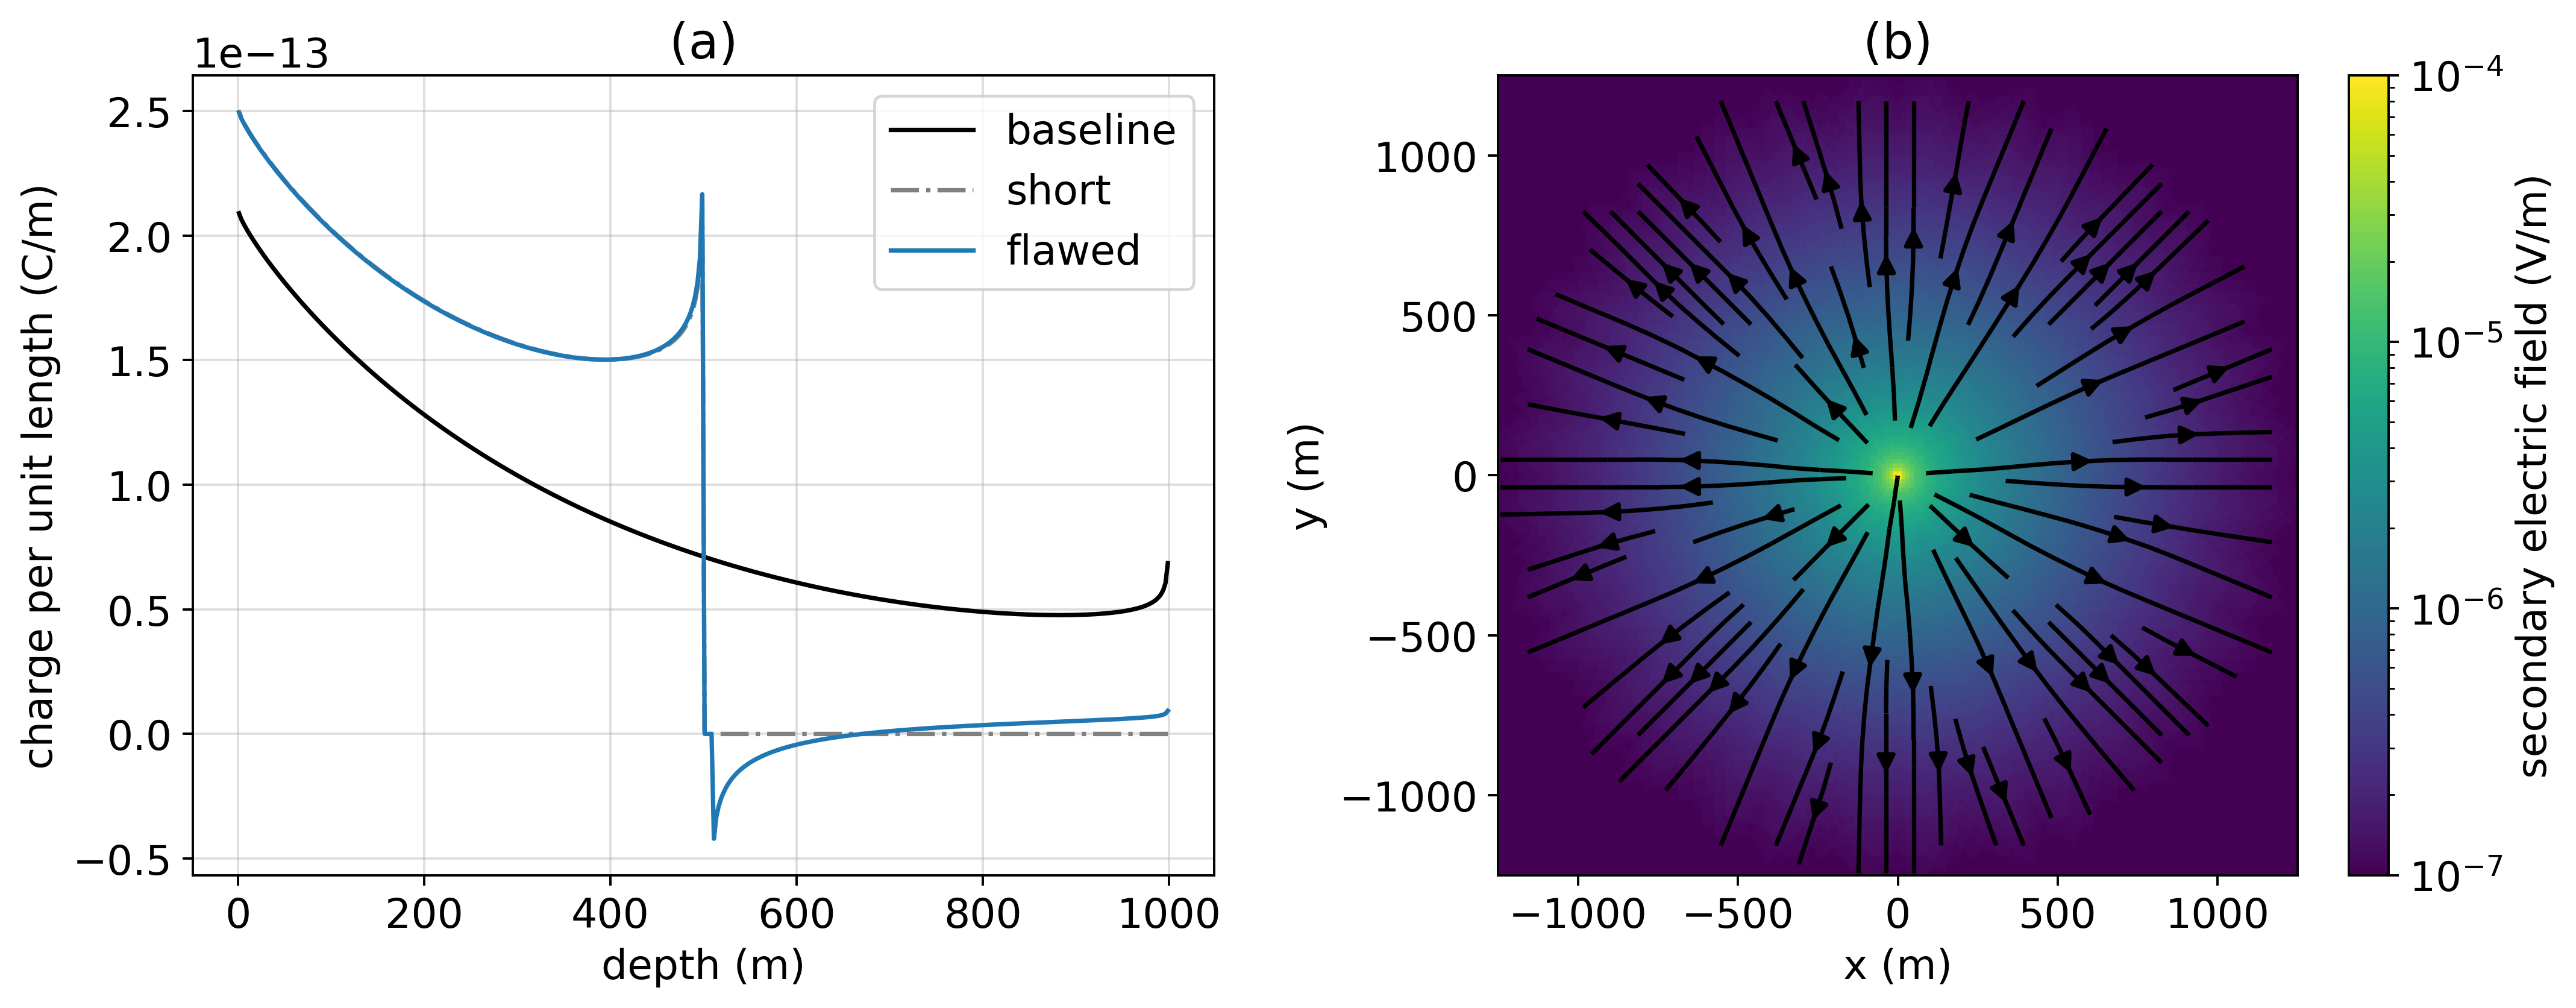
\includegraphics[width=\textwidth]{figures/dc_casing/casing_charge.png}
    \end{center}
\caption{
    (a) Charge along the length of the intact well (black),
    a 500 m well ( ``short'', grey dash-dot), and
    a well with a 10 m flaw at 500 m depth (blue),
    in a top-casing DC resistivity experiment.
    (b) Secondary electric field due on the surface of the earth due to the
    flaw in the casing. The primary is
    defined as the electric field due to the 1000 m long intact well. The return electrode
    is 2000 m away from the well.
}
\label{fig:casing_charge}
\end{figure}
